\section{Results}\label{sec:results}
We assess held-out tracking, distinguish trained-body coverage from unseen
transfer, and use design comparisons and failures to delimit the claim.

\subsection{Tracking held-out motions on trained bodies}\label{sec:test_results}

The epoch-28,170 checkpoint was re-evaluated offline with a standalone
streaming evaluator, once on the validation split and once on the
independent test split. Both runs use the same protocol as training-time
monitoring -- one deterministically selected body shape per clip, an
environment with that exact asset, the mean action, and a capped horizon --
and write a per-motion record for every clip. The test manifest is loaded
only by this standalone evaluator; its SHA-256 and clip count are checked
against the split metadata, and its disjointness from train and validation is
verified before evaluation. All test clips are the standard 6.6\,s HumanML3D
crop, so none reach the horizon cap. The test split is evaluated once; its
number is not iterated against.

\begin{table}[t]
\centering
\small
\caption{Offline evaluation of the epoch-28,170 checkpoint on the 1,048-clip
validation and 1,048-clip test splits of \texttt{hhi\_stage2\_v1}, one
selected trained body per clip (rotating shape panel index 110). Same
standalone evaluator for both.}\label{tab:test_results}
\begin{tabular}{lrr}
\toprule
Metric & Validation & Test \\
\midrule
Success rate (\%) $\uparrow$ & 98.47 & 99.14 \\
Failure rate (gt err $>0.5$) (\%) $\downarrow$ & 1.53 & 0.86 \\
Mean body-position error (m) $\downarrow$ & 0.0699 & 0.0676 \\
Mean global body-rotation error (rad) $\downarrow$ & 0.1738 & 0.1723 \\
Mean maximum-joint position error (m) $\downarrow$ & 0.1419 & 0.1393 \\
Normalized jerk $\downarrow$ & 1,154.3 & 1,050.9 \\
High-jerk windows (\%) $\downarrow$ & 27.46 & 25.33 \\
Worst single clip, gt err max (m) & 3.79 & 1.67 \\
\bottomrule
\end{tabular}
\end{table}

Validation and test scores are similar under the same evaluator. Test
success is 1,039 of 1,048 pairs; validation success is 1,032 of 1,048. No
significance claim is made from their difference. The original test was
revealed once and was not used to select the checkpoint. These scores concern
selected pairs, not every body variant. Continuous pose errors and jerk
complement the permissive 0.5\,m success threshold.

\subsection{Tracking consistency across trained bodies}\label{sec:trained_consistency}
The development replay covers 150 training clips on all 128 trained bodies
(19,200 pairs), with zero failed episodes recorded in the physical analysis.
It establishes broad execution on that training subset, not full-body
coverage of held-out clips evaluated on one body each.

\pending{Replay a frozen held-out subset on all 128 trained bodies. Report
per-clip success fraction, median and worst-body error, and the number of
clips succeeding on every body. Add synchronized reference/controller views
of the same clip across contrasting bodies.}

\subsection{Generalization to unseen bodies}\label{sec:unseen_morphology}
The original epoch-28,170 checkpoint is replayed on 32 bodies excluded from
training: 16 new beta vectors in $[-3,3]^{10}$ instantiated in both male and
female SMPL templates. The panel contains 1,024 clips on every body (32,768
pairs): 932 original training clips isolate the body axis; 47 validation and
45 test clips also have unseen motion identities. Mean-action replay uses
matching assets, a 210-step cap, and the 0.5\,m maximum mean-body-position-error
threshold. Episodes have approximately 198 steps. These references have
frame-zero grounding rather than full training-reference refinement.

\begin{table}[t]
\centering\small
\caption{Original-checkpoint unseen-body replay. The final two rows partition
the full population; they are diagnostic subgroups. Errors are pair means in
metres and radians.}\label{tab:unseen_population}
\begin{tabularx}{\linewidth}{@{}Yrrrr@{}}
\toprule
Population & Pairs & Success (\%) & Position & Rotation \\
\midrule
All 32 bodies & 32,768 & 91.64 & 0.177 & 0.314 \\
Seen clips, all 32 & 29,824 & 91.69 & 0.176 & 0.313 \\
Held-out clips, all 32 & 2,944 & 91.07 & 0.181 & 0.324 \\
Other 28 (all clips) & 28,672 & 99.74 & 0.093 & 0.201 \\
Four severe (all clips) & 4,096 & 34.89 & 0.765 & 1.107 \\
\bottomrule
\end{tabularx}
\end{table}

Overall success is 91.64\%. The other 28 bodies reach 99.74\%, but that
subgroup includes a milder outlier, \texttt{male\_95749fe2}, at approximately
96.3\%. Strong transfer is common but not uniform. The four severe cases
remain part of the overall result.

\begin{table}[t]
\centering\small
\caption{Severe cases on 932 original training clips. Opposite-template
variants share numeric beta vectors but differ in geometry and dynamics.}\label{tab:unseen_flagged}
\begin{tabular}{lrr}
\toprule
Beta key & Severe case, success & Opposite-template success \\
\midrule
\texttt{a83170f5} & male: 58.3\% & female: 100.0\% \\
\texttt{cf3d5ee7} & male: 46.8\% & female: 99.8\% \\
\texttt{4d1b9df1} & female: 35.8\% & male: 99.8\% \\
\texttt{1d4da893} & female: 0.1\% & male: 99.8\% \\
\bottomrule
\end{tabular}
\end{table}

The severe cases show tracking error without recorded termination. Success
on the opposite template suggests a body-specific mechanism, but does not
establish an asset defect: the coefficients map through different templates.
Static inspection found substantial segment-mass differences for three cases,
while \texttt{4d1b9df1} lacked that pattern. Dynamic traces and controlled
interventions are needed to explain the failures.

\begin{figure}[t]
\centering
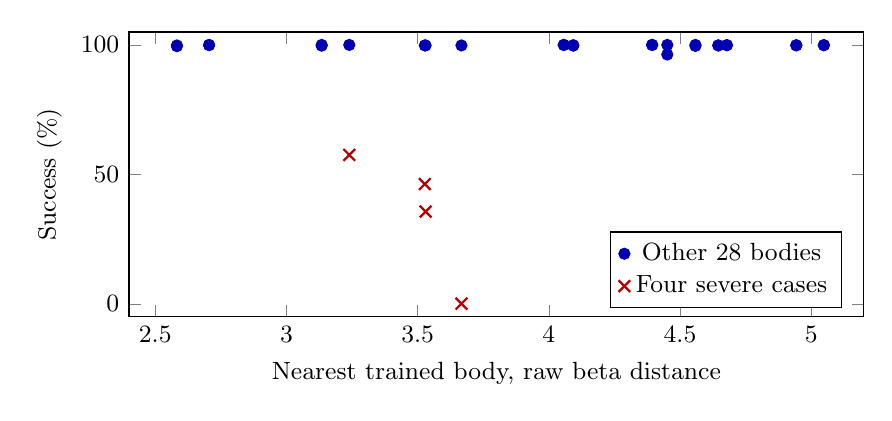
\begin{tikzpicture}
\begin{axis}[
 width=0.9\linewidth,height=5.2cm,
 xlabel={Nearest trained body, raw beta distance},ylabel={Success (\%)},
 xmin=2.4,xmax=5.2,ymin=-5,ymax=105,
 legend pos=south east,legend style={font=\small},
 tick label style={font=\small},label style={font=\small}]
\addplot[only marks,mark=*,blue!70!black] coordinates {
(4.0932,99.7070)
(2.5827,99.8047)
(4.6459,99.8047)
(4.0570,100.0000)
(4.3938,100.0000)
(4.6785,99.9023)
(4.9430,99.9023)
(4.4515,100.0000)
(3.2395,100.0000)
(5.0481,99.9023)
(2.7052,99.9023)
(3.5273,99.8047)
(3.1343,100.0000)
(4.5587,100.0000)
(4.0932,99.9023)
(2.5827,99.5117)
(3.6670,99.8047)
(4.6459,99.8047)
(3.5304,99.8047)
(4.0570,100.0000)
(4.3938,100.0000)
(4.6785,99.9023)
(4.9430,99.8047)
(4.4515,96.2891)
(5.0481,99.9023)
(2.7052,100.0000)
(3.1343,99.7070)
(4.5587,99.6094)
};
\addlegendentry{Other 28 bodies}
\addplot[only marks,mark=x,mark size=3pt,thick,red!70!black] coordinates {
(3.6670,0.0977)
(3.5304,35.6445)
(3.2395,57.5195)
(3.5273,46.2891)
};
\addlegendentry{Four severe cases}
\end{axis}
\end{tikzpicture}
\caption{All 32 unseen bodies, each evaluated on the same 1,024 clips.
Distance uses the nearest trained body of the same SMPL template. The four
severe cases are retained, and success is not uniformly high over the panel.}
\label{fig:unseen_distance}
\end{figure}

Nearest-trained-body distances span approximately 2.58--5.05 in raw beta
coordinates, comparing within template. Figure~\ref{fig:unseen_distance} shows all bodies. The successful subgroup has no clear
descriptive decline over that range; this does not establish full-population
invariance or extrapolation. Explicit conditioning is present, but this study
does not isolate its benefit from shape information in state and references.

\subsubsection{Pending full-data checkpoint comparison}
\pending{Replay the preselected epoch-34,000 full-data checkpoint on the same
32,768 pairs. Include all bodies and report recoveries, regressions, and error
changes. Additional training includes all original motion splits on the
original 128 bodies, so this tests unseen bodies on known motions. Add a
matched trained-body control. No outcome is assumed while GPU evaluation is
unavailable.}

\subsection{Architecture trade-offs across training seeds}\label{sec:architecture_results}
Each refined-reference architecture has three seeds. Each run contributes
one last-eight-evaluation summary (epochs 4,600--6,000); uncertainty below is
sample standard deviation across three summaries. Seed-1/2 values were checked
against local TensorBoard records. Seed-0 values are retained from the
historical table; their original logs were not independently available in that check.

\begin{table}[t]
\centering\small
\caption{Three-seed refined-reference development comparison. Success and
jerk are mean $\pm$ sample standard deviation across seeds; position and
rotation are across-seed means.}\label{tab:architecture_seeds}
\begin{tabularx}{\linewidth}{@{}Yrrrr@{}}
\toprule
Architecture & Success (\%) & Pos. (m) & Rot. (rad) & Jerk \\
\midrule
A: temporal MLP & $95.14\pm2.07$ & 0.118 & 0.216 & $2{,}110\pm643$ \\
B: temporal attention & $97.56\pm0.34$ & 0.090 & 0.218 & $2{,}783\pm887$ \\
C: slot/type attention & $97.89\pm0.22$ & 0.090 & 0.219 & $2{,}413\pm762$ \\
D: C + adaLN-Zero & $97.17\pm0.08$ & 0.083 & 0.211 & $2{,}659\pm674$ \\
\bottomrule
\end{tabularx}
\end{table}

C has the highest mean success; D has the lowest position and rotation errors;
A has the lowest mean jerk. No model dominates. Jerk ordering changes across
seeds, so the apparent factor-of-two advantage in seed 0 is not a consistent
architecture effect. Three seeds do not establish statistical superiority
from small success differences. We retain C as a practical compromise.
These reruns support the already-trained full-scale model rather than
establishing selection before training. Capacities and runtimes differ
(Appendix~\ref{app:history}).

\subsection{Reference refinement: artifact reduction and fidelity}\label{sec:refinement_results}

A paired reference audit supports reduced sliding and penetration with
small pose/root changes, at the cost of higher reference jerk. Policy
comparisons do not establish a causal benefit or absence of quality cost.

The reference-level part is an offline before/after audit on the packaged
motion tensors, with no simulation, over all 19,200 references of the 150-clip
development set (150 clips $\times$ 128 body configurations).
Table~\ref{tab:refine_audit} reports the artifact measures -- stance-foot
horizontal speed during detected contact, the fraction of frames whose lowest
body centre is below the floor, and reference-domain position jerk -- and the
fidelity measures -- per-body geodesic rotation change, root horizontal
displacement, and the cross-shape variance of per-shape knee-flexion range,
which must be preserved rather than flattened.

\begin{table}[t]
\centering
\small
\caption{Reference-refinement audit over all 19,200 development references.
Artifact rows: corpus mean before and after, and the fraction of individual
motions that improve; the per-motion distributions are in
Figure~\ref{fig:refine_dist}. Fidelity rows: corpus mean of the
refined-vs-unrefined difference. Jerk is the raw mean third-difference of body
positions, not the windowed evaluator score.}\label{tab:refine_audit}
\begin{tabularx}{\linewidth}{@{}Yrrr@{}}
\toprule
& Unref.\ mean & Refined mean & Motions improved \\
\midrule
Stance-foot speed (m/s) $\downarrow$ & 0.055 & 0.038 & 96\% \\
Frames below floor (\%) $\downarrow$ & 39.6 & 3.3 & 45\% \\
Frames within 2\,cm of floor (\%) $\downarrow$ & 49.8 & 33.6 & --- \\
Position jerk (m/s$^3$) & 45.2 & 60.7 & 21\% \\
\midrule
Per-body rotation change (deg) & \multicolumn{3}{c}{0.12} \\
Root horizontal displacement (m) & \multicolumn{3}{c}{0.008} \\
Cross-shape var., knee-flexion range (ratio r/u) & \multicolumn{3}{c}{0.94} \\
\bottomrule
\end{tabularx}
\end{table}

\begin{figure}[t]
\centering
\begin{tikzpicture}
\begin{groupplot}[
  group style={group size=2 by 1, horizontal sep=1.4cm},
  width=0.44\linewidth, height=4.6cm,
  boxplot/draw direction=y, xtick={1,2}, xticklabels={unref., refined},
  tick label style={font=\small}, label style={font=\small},
]
\nextgroupplot[ylabel={stance-foot speed (m/s)}, ymin=0, ymax=0.14]
\addplot+[boxplot prepared={lower whisker=0.0174, lower quartile=0.0294,
  median=0.0430, upper quartile=0.0695, upper whisker=0.1228}] coordinates {};
\addplot+[boxplot prepared={lower whisker=0.0078, lower quartile=0.0151,
  median=0.0237, upper quartile=0.0476, upper whisker=0.1157}] coordinates {};
\nextgroupplot[ylabel={position jerk (m/s$^3$)}, ymin=0, ymax=170]
\addplot+[boxplot prepared={lower whisker=6.5, lower quartile=14.0,
  median=30.4, upper quartile=61.6, upper whisker=133.5}] coordinates {};
\addplot+[boxplot prepared={lower whisker=5.7, lower quartile=20.8,
  median=49.2, upper quartile=86.7, upper whisker=161.6}] coordinates {};
\end{groupplot}
\end{tikzpicture}
\caption{Per-motion distributions (box: quartiles; whiskers: 5th--95th
percentile) over the 19,200 development references. Foot-skate drops across
almost the whole distribution; position jerk rises across almost the whole
distribution.}\label{fig:refine_dist}
\end{figure}

Refinement removes most ground penetration and about a third of the
stance-foot sliding, while changing joint rotations by a tenth of a degree
and the root path by millimetres, and leaving the cross-shape spread of
per-shape knee kinematics essentially intact (variance ratio 0.94). The
per-motion distributions (Figure~\ref{fig:refine_dist}) show these are not
mean-only effects: stance-foot speed falls for 96\% of individual motions,
across the full range rather than a few outliers, although the worst-sliding
5\% of clips are barely improved. Penetration in the raw references is
bimodal -- a large fraction of clips sit entirely below the floor, a
whole-clip vertical mis-registration rather than per-frame jitter, which the
clearance correction removes; clips that were already grounded stay grounded,
so only 45\% of motions register a change. The cost is a roughly one-third
increase in reference-domain position jerk that is broad rather than
tail-driven: 79\% of motions get jerkier, and the effect is a clip property,
not a shape property. Grouped by clip (150), the median jerk moves 30.8 to
50.9 and the range spans 3.9--237 (unrefined) versus 3.4--246 (refined);
grouped by body shape (128), the medians move 45.5 to 60.5 within a tight
36--57 versus 51--74 band, so refinement raises jerk almost uniformly across
morphologies. It is introduced by the per-window root-translation correction
and the per-frame ground-clearance lift. Higher target jerk could contribute to the lower policy jerk of the
unrefined slot/type seed-0 run, but different targets and training variability
prevent attribution to references alone.

The refined/unrefined pairs in Table~\ref{tab:ablation_results} track their
own targets and have one seed per unrefined case. They describe different
tasks. The reference audit justifies cleaning; a stronger policy-level claim
requires a common-reference checkpoint comparison.

\subsection{Residual failure patterns}\label{sec:failures}
Nine test pairs and 16 validation pairs fail the configured threshold.
Caption joins suggest ground transitions (six test, five validation failures)
and whole-body rotations (two test, four validation failures). These describe
the failed sample rather than mechanical causes. Without class counts among
successful clips they do not establish class-specific failure rates.

Other captions describe turning, side-stepping, an abrupt stop, and a hand-held
sparring stick absent from simulation. An omitted object does not establish
missing load-bearing support. A clip with rounded peak error near 0.5\,m
remains in the failure count pending exact threshold sensitivity. Failures in
both orientations on different bodies do not isolate skill, morphology, or
reference effects.

\pending{Inspect synchronized rollouts and first-crossing traces, including
successful variants of the same clips. Use population class denominators
before claiming enrichment and interventions before assigning causes.}
